% !TEX root = ../thesis-sample.tex

\chapter{Experimental Results}\label{chap:Experiments}

In this chapter, we present three experiments that demonstrate the efficacy of the proposed exact occupancy grid mapping and autonomous exploration from earlier chapters. The first example involves a ground vehicle mapping and exploring a 2D space. The second example is a quadrotor unmanned aerial vehicle (UAV) flying around a vertically-uniform space while generating a 3D map from level flight. The final example shows autonomous exploration completely in 3D, where a quadrotor must map and explore around complicated objects.

\section{Pioneer Ground Vehicle Tests}
\label{sec:PioneerNRL}

The experiment involves a ground vehicle producing a probabilistic occupancy grid map in real time. The robot motion is governed by the information gain-maximizing policy described in Chapter \ref{chap:ae2D}.


\paragraph{Hardware Configuration}
The Pioneer 3 ground robot is chosen for this experiment because of its reliability and simple operation. The vehicle accepts two inputs, namely linear velocity (aligned with the robot wheels) and angular velocity (about a central axis passing vertically through the robot). The robot pose is estimated via Vicon Tracker, which provides the location and attitude of a rigid body. The depth readings are obtained by a Kinect depth sensor. Since the experiment is to map and explore a 2D environment, only a single central row of the 3D Kinect depth scan provide the necessary measurements. The robot captures an experimental environment with walls constructed from Styrofoam.

\paragraph{Software Configuration}

The software structure is similar to ROS nodes Section \ref{sec:Ae2DNumExamples}, which simply involves a mapping node, an exploration node, and a visualization node using ``OpenGL'' libraries. The only differences are eliminating the simulator (Stage) and adding synchronization among the sensors, which is of high importance to the proposed occupancy grid mapping approach. Any time delay between the robot pose estimation and the sensor depth readings can cause conflicting information, which may be harmful to the probabilistic map. Thus, ROS approximate message filters are applied such that the pose from Vicon Tracker ($100$Hz) and the Microsoft Kinect ($30$Hz) are nearly synchronized, which provides validity of the assumption that the measurement ray positions and directions are known deterministically.

\paragraph{Exploring and Mapping a 2D Environment}
The environment consists of Styrofoam walls on a flat floor. The perimeter is rectangular, with several obstacles and angled walls (see Figure \ref{fig:ExpSetupPhoto}). The robot autonomously explored the space using the complete Cartesian searching approach, and Dijkstra's algorithm provides collision-free waypoints to the optimal future poses. Based on these waypoints, a constrained least squares polynomial fitting generates a smooth trajectory to follow the waypoints with fixed velocity. Finally, a simple controller is implemented such that the Pioneer follows the trajectory by moving and orienting toward the desired robot location $1$ sec in the future.

\begin{figure}
	\centering
    	\begin{subfigure}[b]{0.45\textwidth}
        		\includegraphics[width=\textwidth]{test_setup_bottom_left_cropped.jpg}
        		\caption{Bottom-left view}
        		\label{fig:Experiment_blv}
    	\end{subfigure}
	\hspace*{0.05\columnwidth}
	\begin{subfigure}[b]{0.45\textwidth}
        		\includegraphics[width=\textwidth]{test_setup_bottom_right_cropped.jpg}
        		\caption{Bottom-right view}
        		\label{fig:Experiment_brv}
    	\end{subfigure}
\caption{Images from two perspectives show the walls and obstacles of the experimental environment.}
\label{fig:ExpSetupPhoto}
\end{figure}


The resulting occupancy grid maps and trajectories are depicted in Figure \ref{fig:ExperimentOGM} and a video is available at \href{https://www.youtube.com/watch?v=CRQfhhICSj0&feature=youtu.be}{\WriteBlue{www.youtube.com/watch?v=CRQfhhICSj0\&feature=youtu.be}}. Most importantly, the robot builds a clear occupancy grid map despite sensor noise and imperfect sensor synchronization. The autonomous exploration successfully guides the robot such that it builds a map of the reachable space without colliding with any obstacles.


\begin{figure}
	\centering{
    	\begin{subfigure}[b]{0.19\textwidth}
        		\includegraphics[trim={13cm 1cm 13cm 0}, clip, width=\textwidth]{feb23_t0sec.jpg}
        		\caption{$t=0$ sec}
        		\label{fig:Experiment_ogm_t0}
    	\end{subfigure}
	\begin{subfigure}[b]{0.19\textwidth}
        		\includegraphics[trim={13cm 1cm 13cm 0}, clip, width=\textwidth]{feb23_t20sec.jpg}
        		\caption{$t=20$ sec}
        		\label{fig:Experiment_ogm_t0p5}
    	\end{subfigure}    
	\begin{subfigure}[b]{0.19\textwidth}
        		\includegraphics[trim={13cm 1cm 13cm 0}, clip, width=\textwidth]{feb23_t40sec.jpg}
        		\caption{$t=40$ sec}
        		\label{fig:Experiment_ogm_t1}
    	\end{subfigure}
	\begin{subfigure}[b]{0.19\textwidth}
        		\includegraphics[trim={13cm 1cm 13cm 0}, clip, width=\textwidth]{feb23_t60sec.jpg}
        		\caption{$t=60$ sec}
        		\label{fig:Experiment_ogm_t1p5}
    	\end{subfigure}
	\begin{subfigure}[b]{0.19\textwidth}
        		\includegraphics[trim={13cm 1cm 13cm 0}, clip, width=\textwidth]{feb23_t80sec.jpg}
        		\caption{$t=80$ sec}
        		\label{fig:Experiment_ogm_t2}
    	\end{subfigure}
		\vspace*{0.05\textwidth}

	}
	\centering{
    	\begin{subfigure}[b]{0.19\textwidth}
        		\includegraphics[trim={13cm 1cm 13cm 0}, clip, width=\textwidth]{feb23_t100sec.jpg}
        		\caption{$t=100$ sec}
        		\label{fig:Experiment_ogm_t2p5}
    	\end{subfigure}
	\begin{subfigure}[b]{0.19\textwidth}
        		\includegraphics[trim={13cm 1cm 13cm 0}, clip, width=\textwidth]{feb23_t120sec.jpg}
        		\caption{$t=120$ sec}
        		\label{fig:Experiment_ogm_t3}
    	\end{subfigure}    
	\begin{subfigure}[b]{0.19\textwidth}
        		\includegraphics[trim={13cm 1cm 13cm 0}, clip, width=\textwidth]{feb23_t140sec.jpg}
        		\caption{$t=140$ sec}
        		\label{fig:Experiment_ogm_t3p5}
    	\end{subfigure}
	\begin{subfigure}[b]{0.19\textwidth}
        		\includegraphics[trim={13cm 1cm 13cm 0}, clip, width=\textwidth]{feb23_t160sec.jpg}
        		\caption{$t=160$ sec}
        		\label{fig:Experiment_ogm_t4}
    	\end{subfigure}
	\begin{subfigure}[b]{0.19\textwidth}
        		\includegraphics[trim={13cm 1cm 13cm 0}, clip, width=\textwidth]{feb23_t180sec.jpg}
        		\caption{$t=180$ sec}
        		\label{fig:Experiment_ogm_t4p5}
    	\end{subfigure}
	}
\caption{A robot autonomously explores the experimental environment and produces an occupancy grid map along the way. The robot (shaded green circle body with shaded blue circle sensor) is controlled toward the desired pose $1$ sec in the future (unshaded grey robot), which is following a constrained least-squares trajectory (cyan curve). This trajectory is based on waypoints (black circles) from Dijkstra's algorithm to arrive at the optimal pose (unshaded green circle body with unshaded blue circle sensor) as proposed in this paper.}
\label{fig:ExperimentOGM}
\end{figure}

The resulting map and exploration commands are generated in real time. The grid cells are stored as double-float variables in a vector, where the vector index is mapped to a location on the occupancy grid. Thus, the memory requirements are proportional to the number of grid cells, which is roughly the mapping area divided by the area of a grid cell. Since cell locations need not be saved because the mapping between cell index and location is known, memory requirements are reduced. On a Lenovo T540p laptop with an Intel Core i7-4900MQ processor (quad-core, 2.8GHz per core) and 16GB of RAM, the mean time for updating the occupancy grid is $0.0115$ seconds, and the mean time to determine an exploration strategy is $0.6820$ seconds. Time requirements for mapping and exploration are easily modified by changing grid cell resolution or the number of exploration pose candidates, respectively. In short, there is a tradeoff between computational speed and accuracy of mapping or exploration.

The autonomous exploration is governed by a policy to maximize expected entropy decreases, so entropy and entropy change with time (Figure \ref{fig:ExperimentH}) are important metrics. In this example, the a priori occupancy probabilities of all cells are $0.1$, so the entropies could temporarily rise for likely occupied cells. The total map entropy begins at roughly $2613$ and decreases by roughly half to $1338$. Many grid cells within the map limits are occluded by walls, preventing the blocked cells from occupancy probability changes. In some cases, the robot is able to update the cell occupancy probabilities; in other cases, cells fall inside regions occluded from all reachable space, and the robot cannot update these cells. Among those grid cells visible from collision-free locations, the vast majority of cells were updated in less than $3$ min while following a very slow ($5$ cm/sec) trajectory.

In conclusion, this example shows how occupancy grid mapping and autonomous exploration are applied to a ground vehicle in a 2D environment such as a floor of a house or building. Dijkstra's search is applied about the occupancy grid, and a smooth trajectory is easily tracked with a simple controller that tracks a polynomial least squares trajectory. These results show the efficacy of exact occupancy grid mapping and autonomous exploration. Next, we extend these experiments to 3D.

\begin{figure}
	\centering
	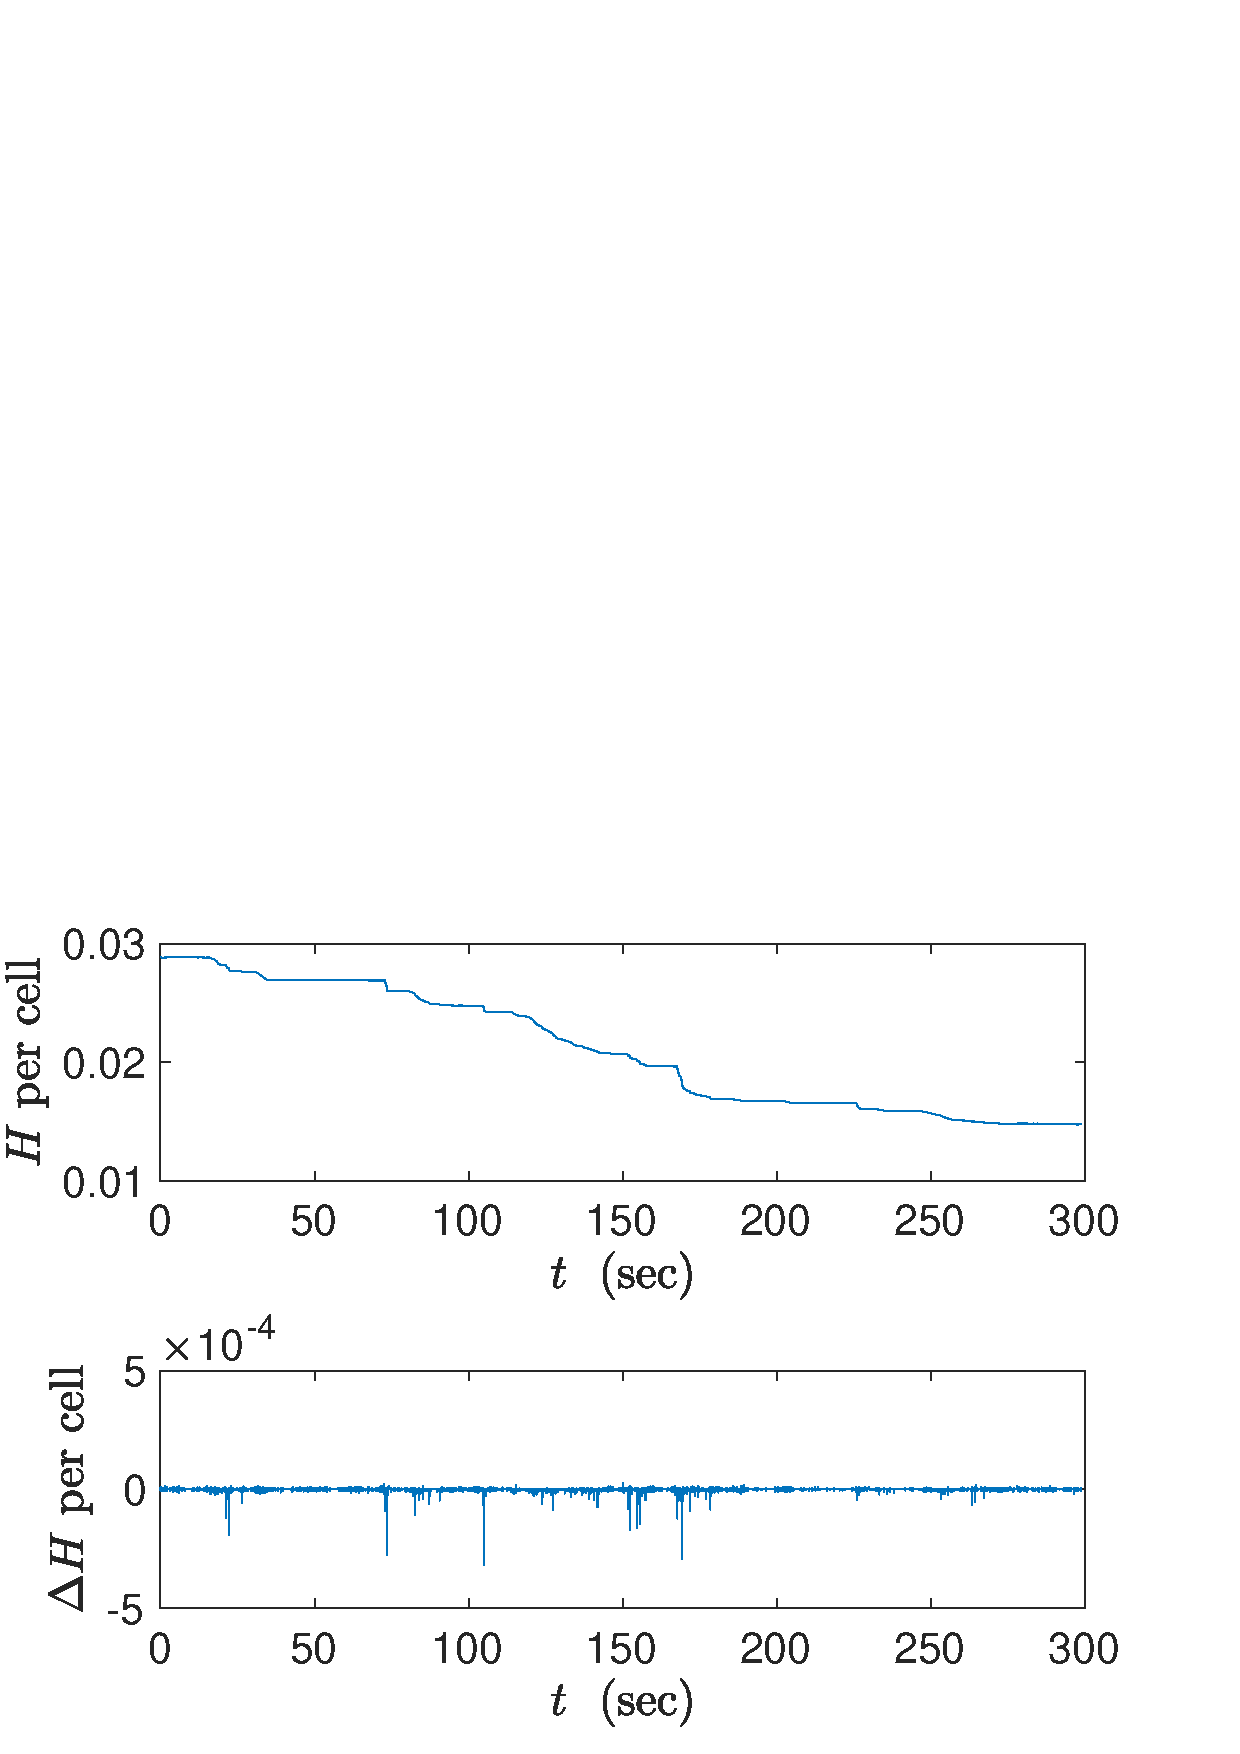
\includegraphics[width=\textwidth]{JIRS_fig11.pdf}
	\caption{The map entropy $H$ averaged over all $90601$ grid cells is reduced during experimentation. The quick changes $\Delta H$ per cell correspond to map updates when the robot captures new territory.}
\label{fig:ExperimentH}
\end{figure}


\section{Quadrotor Exploration of a Large Room}
\label{sec:QuadrotorNRL}

\section{Quadrotor 3D Exploration}
\label{sec:QuadrotorSEH}




